% Finished July 18, 2013
% Put into format of VUW Thesis on March 20, 2014.
% Cut out of Chapter 6 and formed into Appendix E on Monday, 24 March 2014.

\documentclass[12pt, a4paper, twoside, openright]{book}

\usepackage{vuwthesis} % sets up some local things, mostly the front page

\setlength{\intextsep}{12pt} % set space above and below in-line float
\setlength{\abovecaptionskip}{0pt} % set space between figure and caption.


\usepackage{amssymb, amsmath}
%\usepackage{mathtools}
\usepackage{tikz}
\usetikzlibrary{calc}

\newcommand{\beff}{\ensuremath{b_{\mathrm{eff}}}}
\newcommand{\bhom}{\ensuremath{b_{\mathrm{hom}}}}

%\usepackage{marvosym}

\usepackage{etoolbox}
\newtoggle{compilealone}
\toggletrue{compilealone}

\title{Appendix F: Periodic Functions Weakly Converge To Their Mean}
\author{Nat Lund}

\begin{document}
\chapter{Periodic Functions Weakly Converge To Their Mean}\label{C:weakconvergence}

In this Appendix we prove that periodic functions weakly converge to their mean, a fact we use in Chapter 6.  To keep the Appendix self-contained, we start by defining weak convergence, using the definitions duplicated in Chapter 6.

\clearpage
\section{Weak Convergence}

Consider a sequence of functions defined by:
\begin{equation}
f_n = \sin(n x)
\end{equation}
the first three functions of which appear in Figure (\ref{sinnx}).
\begin{figure}[ht]
\centering
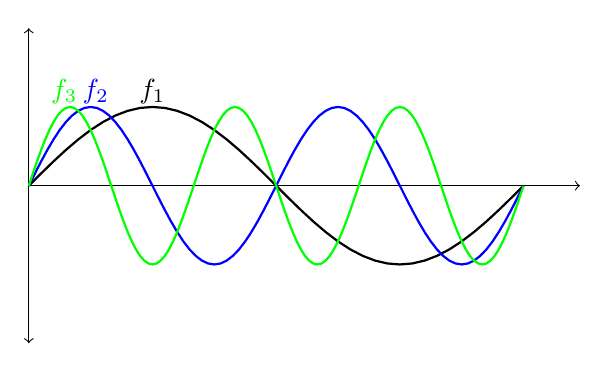
\begin{tikzpicture}

\draw[->] (0,0) -- (7,0);
\draw[<->] (0,-2) -- (0,2);

% samples = 4n per period + 1. n is resolution
\draw [thick, domain=0:6.283,samples=41] plot (\x, { sin(\x  r) });
\draw [color=blue,thick, domain=0:6.283, samples=81] plot (\x, { sin(2*\x  r) });
\draw [color=green,thick, domain=0:6.283, samples=121] plot (\x, { sin(3*\x r) });

\node at (1.57,1.2) {$f_1$};
\node at (0.85,1.2) [color=blue] {$f_2$};
\node at (0.45,1.2) [color=green] {$f_3$};

%\draw[color=red,thick, samples=97, domain=1:5] plot (\x, { 0.2 * sin( 3*pi*(\x-1) r) } );

\end{tikzpicture}
\caption{The first three functions in the sequence $\sin (n x)$.}\label{sinnx}
\end{figure}

As $n$ increases, the period of the sine wave gets smaller and smaller, but the amplitude is unchanged.  In the limit as $n \to \infty$, the waveform gets infinitely `spiky'.  What does the sequence converge to?  There is no intuitive sense of the sinewave sequence getting `closer to' some limit function.  In fact, the sequence does not strongly converge.

However, there is a sense in which the function sequence converges. 

We multiply each function in the sequence by an arbitrary test function $g$, and integrate, thus creating a sequence of integrals:
\begin{equation}
\int g f_n \;dx
\end{equation}
If the sequence of integrals (strongly) converges to a limit integral:
\begin{equation}
\int g f_n \;dx \to \int g f \;dx
\end{equation}
then we say that $f_n$ \textbf{weakly converges} to $f$, and the `limit function' $f$ appearing in the limit integral is known as the \textbf{weak limit.}  This is also written:
\begin{equation}
f_n \rightharpoonup f
\end{equation}
%What is the weak limit $f$?  
%If $f_n$ is a sequence of periodic functions (like our sine wave example) then $f$ is the \textbf{mean} of $f_n$, denoted $\left< f_n \right>  $.

%We shall prove (and use) this incredibly useful result.

\subsection{Periodic Functions Weakly Converge to their Mean}

It is a `standard result' that periodic functions weakly converge to their mean.  In a 2002 paper \cite{Lukkassen2002}, Lukkassen and Wall state: ``We have not found proofs of [this] fact in the literature.  The aim of this paper is to present such proofs."  Their paper provides a rigorous proof (and generalization) of this proof.  Here, however, we present a simple intuitive proof, suitable for this thesis.

\vspace{1em}

Consider our example of a sine wave sequence, together with an arbitrary test function $g$, integrated over the domain $0$ to $2 \pi$.
Each integral in the sequence is of the form:
\begin{equation}
\int_0^{2\pi} g(x) \sin(nx) \;dx
\end{equation}
Over the domain $0$ to $2\pi$, the function $\sin(nx)$ has exactly $n$ periods, each of width $2\pi /n$.
We chop up the integral into $n$ separate integrals, each with a subdomain of width $2\pi/n$.
\begin{equation}
\sum_{k=1}^n  \int_{(k-1) \frac{2\pi}{n}}^{k \frac{2\pi}{n}} g(x) \sin(nx) \;dx
\end{equation}
This is shown in Figure (\ref{sineg}).
\begin{figure}[ht]
\centering
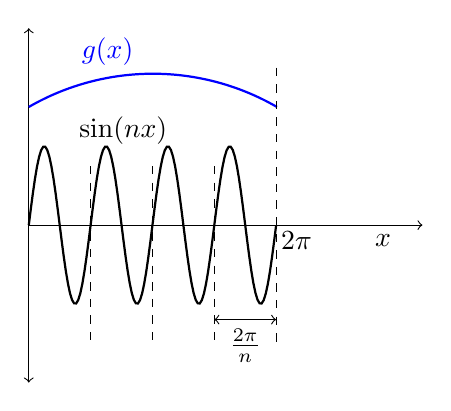
\begin{tikzpicture}

\draw[->] (0,0) -- (5,0);
\draw[<->] (0,-2) -- (0,2.5);
\node at (4.5,0) [below] {$x$};


% samples = 4n per period + 1. n is resolution
\draw [thick, domain=0:3.1416, samples=121] plot (\x, { sin(4*\x*2 r) });

\draw [color=blue, thick] (0,1.5) arc (120:60:3.1516 cm);

\node at (1.2,1.2) {$\sin(nx)$};
\node at (1,2.2) [color=blue] {$g(x)$};

\node at (3.4,-0.2) {$2\pi$};

\draw[dashed] (3.1416,2) -- ++(0,-3.5);
\foreach \k in {1,2,3}
{\draw[dashed] (\k*3.1416/4, 0.75) --++(0,-2.25);}

\draw[<->] (3.1416,-1.2) -- node[below] {$\frac{2\pi}{n}$} ++(-3.1416/4, 0);


\end{tikzpicture}
\caption{The periodic function $\sin (nx) $ and test function $g(x)$.}\label{sineg}
\end{figure}

\clearpage
By a change of variable, we `stretch' the domain so that in terms of the new variable, the period of the sine wave is again $2\pi$.  The domain is dilated by factor $n$ and now has width $2\pi n$. 
With change of variable $x = t/n$, we have $dx = 1/n \,dt$.  Pulling the Jacobian $1/n$ out of the sum, we have:
\begin{equation}
\frac{1}{n} \sum_{k=1}^n  \int_{(k-1) 2\pi}^{k 2\pi} g \left(\frac{t}{n} \right) \sin(t) \;dt 
, \qquad x = \frac{t}{n}, \quad dx = \frac{1}{n} dt
\end{equation}
Put another way, we move the $n$ dependence from the sine function to the test function $g$.  See Figure (\ref{dilate}).

\begin{figure}[ht]
\centering
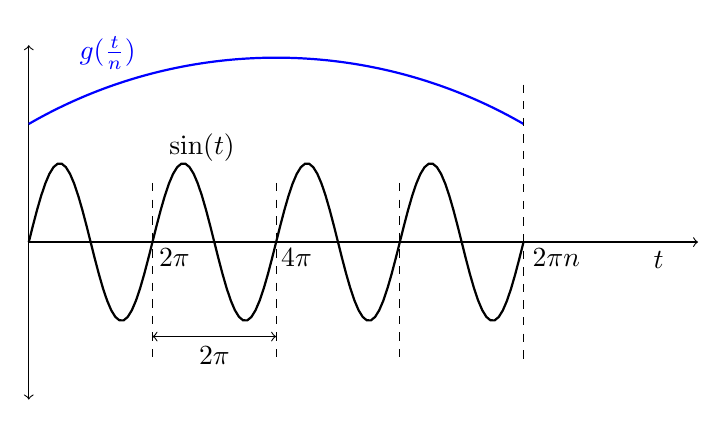
\begin{tikzpicture}

\draw[->] (0,0) -- (8.5,0);
\draw[<->] (0,-2) -- (0,2.5);
\node at (8,0) [below] {$t$};

% samples = 4n per period + 1. n is resolution
\draw [thick, domain=0:6.283, samples=121] plot (\x, { sin(4*\x r) });

\draw [color=blue, thick] (0,1.5) arc (120:60:6.283 cm);

\node at (2.2,1.2) {$\sin(t)$};
\node at (1,2.4) [color=blue] {$g(\frac{t}{n})$};

\node at (1.85,-0.2) {$2\pi$};
\node at (3.4,-0.2) {$4\pi$};
\node at (6.7,-0.2) {$2\pi n$};

\draw[dashed] (6.283,2) -- ++(0,-3.5);
\foreach \k in {1,2,3}
{\draw[dashed] (\k*3.1416/2, 0.75) --++(0,-2.25);}

\draw[<->] (3.1416,-1.2) -- node[below] {$2\pi$} ++(-3.1416/2, 0);


\end{tikzpicture}
\caption{Change of variable dilates the domain.}\label{dilate}
\end{figure}

%Even more cunningly, 
We note that a period of $\sin(t)$ is the same for all $k$, so we use \emph{only} the integral from $0$ to $2\pi$, and `transport' the appropriate bit of $g(t)$ back to the interval $0$ to $2\pi$.  This is accomplished by adding $(k-1) (2\pi /n)$ to the argument of $g(t/n)$.  For clarity, we shall change variables again, $t \to \xi$, to highlight the fact that while the domain of $t$ is the interval $0$ to $2\pi n$, the domain of $\xi$ is only the interval $0$ to $2\pi$.
\begin{equation}
\frac{1}{n} \sum_{k=1}^n  \int_0^{2\pi} g\left(\frac{\xi}{n} + (k-1) \frac{2\pi}{n} \right) \sin(\xi) \;d\xi , \qquad x = \frac{\xi}{n}
\end{equation}
The reduced domain is shown in Figure (\ref{reduced}).

\clearpage
\begin{figure}[ht]
\centering
\begin{tikzpicture}

\draw[->] (0,0) -- (8.5,0);
\draw[<->] (0,-2) -- (0,2.5);
\node at (8,0) [below] {$\xi$};

% samples = 4n per period + 1. n is resolution
\draw [thick, domain=0:1.5708, samples=32+1] plot (\x, { sin(4*\x r) });

\draw [dashed,color=blue, thick] (0,1.5) arc (120:60:6.283 cm);
\draw [color=blue, thick] (0,1.5) arc (120:104:6.283 cm);

\node at (0.7,1.2) {$\sin(\xi)$};
\node at (1,2.4) [color=blue] {$g(\frac{\xi}{n})$};

\node at (1.85,-0.2) {$2\pi$};
%\node at (3.4,-0.2) {$4\pi$};
%\node at (6.7,-0.2) {$2\pi n$};

%\draw[dashed] (1.5708,2) -- ++(0,-3.5);
%\draw[dashed] (6.283,2) -- ++(0,-3.5);
\foreach \k in {1,2,3,4}
{\draw[dashed] (\k*3.1416/2, 2.5) --++(0,-3);}

%\draw[<->] (3.1416,-1.2) -- node[below] {$2\pi$} ++(-3.1416/2, 0);


\end{tikzpicture}
\caption{Reduced domain with $g$ parameterised by $k$.}\label{reduced}
\end{figure}

So we have:
\begin{equation}
\frac{1}{n}   \int_0^{2\pi} g\left(\frac{\xi}{n}\right) \sin(\xi) \;d\xi
 + \frac{1}{n}   \int_0^{2\pi} g\left(\frac{\xi + 2\pi}{n} \right) \sin(\xi) \;d\xi
 + \cdots
\end{equation}
%The sum can go under a single integral sign:
%\begin{equation}
%\frac{1}{n}
%\int_0^{2\pi} g\left(\frac{\xi}{n}\right) \sin(\xi)
% + g\left(\frac{\xi + 2\pi}{n} \right) \sin(\xi) 
% + g\left(\frac{\xi + 4\pi}{n} \right) \sin(\xi) + \cdots \;d\xi
%\end{equation}
%And multiplication distributes over addition, so this is:
%\begin{equation}
%\frac{1}{n} \int_0^{2\pi} \sin(\xi)
%\left[
%g\left(\frac{\xi}{n} \right) + g\left(\frac{\xi + 2\pi}{n} \right)  +  
%g\left(\frac{\xi + 4\pi}{n} \right) + \cdots 
%\right] \;d\xi
%\end{equation}
%Or:
The sum can go under a single integral sign, and the $\sin(\xi)$ common factor can be pulled out of the sum:
\begin{equation}
\frac{1}{n} \int_0^{2\pi} \sin(\xi)
 \sum_{k=1}^n g\left(\frac{\xi + (k-1) 2\pi}{n} \right) \;d\xi
\end{equation}
For later convenience, introduce a $2\pi$ and shift the $1/n$ factor:
\begin{equation}
\frac{1}{2\pi} \int_0^{2\pi} \sin(\xi) \;
 \sum_{k=1}^n g\left(\frac{\xi + (k-1) 2\pi}{n} \right) \frac{2\pi}{n} \;d\xi
 \end{equation}

What happens as $n \to \infty$?  The summation term can be written:
\begin{equation}
\sum_{k=1}^n g\left((k-1)\frac{ 2\pi}{n} + \frac{\xi}{n} \right) \frac{2\pi}{n}
 \end{equation}
Since $\xi$ is between $0$ and $2\pi$, the $\xi/n$ term is between $0$ and $2\pi/n$.
As $k$ ranges from $1$ to $n$, the $g(k)$ term provides $n$ `samples' of the function at discrete points a distance $2\pi/n$ apart, with the starting point offset from $0$ by the amount $\xi/n$.  Each sample $g(k)$ is multiplied by the width of the inter-sample distance, giving $n$ rectangles to sum up.   In the limit $n \to \infty$, this is one definition of the Riemann integral of $g$ over the interval $2\pi$.
\begin{equation}
\lim_{n \to \infty} \sum_{k=1}^n g\left((k-1)\frac{ 2\pi}{n} + \frac{\xi}{n} \right) \frac{2\pi}{n} = \int_0^{2\pi} g(x) \;dx
 \end{equation}
The geometry of this Riemann integral is depicted in Figure (\ref{riemann}).
\begin{figure}[ht]
\centering
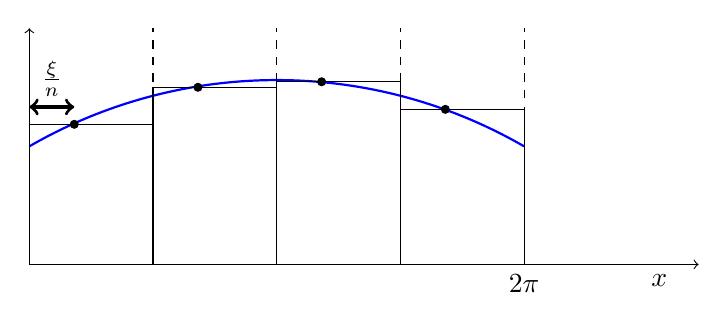
\begin{tikzpicture}
\draw[->] (0,0) -- (8.5,0);
\draw[->] (0,0) -- (0,3);
\node at (8,0) [below] {$x$};
\node at (6.283,0)[below] {$2\pi$};

\draw [color=blue, thick] (0,1.5) arc (120:60:6.283 cm);

\foreach \k / \y in {1 /1.78, 2/2.25, 3/2.32, 4/1.97}
{\draw[dashed] (\k*3.1416/2, 0) -- ++(0,3);
\draw (\k*3.1416/2,\y) rectangle (\k*3.1416/2 - 3.1416/2,0);
\draw[fill] (\k*3.1416/2 - 1, \y) circle (0.5mm); }

\draw[<->,very thick] (0,2) -- node[above]{$\frac{\xi}{n}$} ++(0.571,0);

\end{tikzpicture}
\caption{The geometry of the Riemann integral of $g$.}\label{riemann}
\end{figure}


Thus we have:
\begin{equation}
\frac{1}{2\pi} \int_0^{2\pi} \sin(\xi)
\int_0^{2\pi} g(x) \;dx \;d\xi
= 
\left( \frac{1}{2\pi} \int_0^{2\pi} \sin(\xi) \;d\xi \right)
\left( \int_0^{2\pi} g(x) \;dx \right)
 \end{equation}
Now the integral with the sine function defines the \textbf{mean} of a function:
\begin{equation}
\left< \sin(x) \right> = \frac{1}{2\pi} \int_0^{2\pi} \sin(\xi) \;d\xi
\end{equation}
Therefore, we have shown that:
\begin{equation}
\lim_{n \to \infty} \int_0^{2\pi} g(x) \sin(nx) \;dx = \left< \sin(x) \right>
 \int_0^{2\pi} g(x) \;dx
\end{equation}
Or:
\begin{equation}
\int_0^{2\pi} g(x) \sin(nx) \;dx  \to  
 \int_0^{2\pi} g(x) \left< \sin(x) \right> \;dx
\end{equation}

The mean of $\sin(x)$ happens to be zero, so the limit vanishes.  But the foregoing argument holds for \emph{any} periodic function.  Therefore we have shown that \textbf{periodic functions weakly converge to their mean:}
\begin{equation}
\int g f_n \;dx \to \int g \left< f \right> \;dx
\end{equation}



\iftoggle{compilealone}
    {
    \bibliography{Lund_Thesis.bib}
    \bibliographystyle{plain}
    }

\end{document}
